\documentclass[professionalfont]{beamer}

\usepackage[T1]{fontenc}
\usepackage{amsmath}
\usepackage{graphicx}
\graphicspath{{figures/}}
\usepackage{tikz}

\DeclareMathOperator*{\argmin}{argmin}

% usage: \tikzpic{<x percent>}{<y percent>}{<image size>}{<image name>}
\newcommand*{\tikzpic}[4]{%
\begin{tikzpicture}[remember picture,overlay]
\node at (current page.south west) [xshift=#1\paperwidth,yshift=#2\paperheight] {\includegraphics[width=#3\linewidth]{#4}};
\end{tikzpicture}%
}
\newcommand{\lenitem}[2][.7\linewidth]{\parbox[t]{#1}{\strut #2\strut}}

\title[Hessian-free optimization]{\textbf{\\Hessian-free optimization \\ (Truncated-Newton family)}}
\author[A. Sessa]{\underline{Andrea Sessa} \\ \small{Mat. 850082} \\
\vspace{1mm}
{\small \href{}{\nolinkurl{}}}\\
{\textbf{Optimization - Prof. E. Amaldi} \\ \textit{AA. 2016/2017}}}
\date{}

\usetheme{POLIMI}

\expandafter\def\expandafter\insertshorttitle\expandafter{\insertshorttitle\hfill\insertframenumber\,/\,\inserttotalframenumber}


\begin{document}

  \begin{frame}[plain]
    \titlepage
  \end{frame}

  \section{Introduction}

  \subsection{Motivations}
  \begin{frame}
	\frametitle{Motivations}
  Old methods:
    \begin{itemize}
      \item \textbf{Gradient Descent}: It uses only first order information! Curvature properties
        of the function is ignored.
      \item \textbf{Newton Method}: Second order information are taken into consideration but
        it does not scale well for large instance problems (ie. deep neural nets.)
    \end{itemize}
    Many solution have been proposed in literature (Conjugate-gradient method, Quasi-Newton methods etc.).\newline\newline
    In this presentation we describe a family of methods known as Hessian-free (or Truncated-Newton).\newline\newline
    Moreover we propose an application of such method in the training of \textit{Deep Neural networks}.\newline

  \end{frame}

  \section{Formalization}

  \subsection{Newton Method - Recap - 1}
	\begin{frame}
  	 \frametitle{Newton Method - Recap - 1}
     Let $f \in \mathcal{C}^2$ and $B = H(x)$ with $x \in \mathbb{R}^n$\newline
     The problem is:
     \begin{equation*}
     \begin{aligned}
       & \underset{x}{\text{min}}
       & & f(x) \\
       & \text{st.}
       & & x \in \mathbb{R}^n
     \end{aligned}
     \end{equation*}
     We consider the quadratic approximation of $f$ at $x_k$:
     \begin{equation*}
       q_k(\underline{x}) := f(\underline{x}_k) + \nabla^{t}f(\underline{x}_k)(\underline{x} - \underline{x}_k) + \frac{1}{2}(\underline{x} - \underline{x}_k)^{t}H(\underline{x}_k)(\underline{x} - \underline{x}_k)
     \end{equation*}
     We search for the direction $\underline{d}$ that minimizes $q_k$.\newline
     In particular for the Newton method we have:
     \begin{equation*}
       \underline{d} = H^{-1}(\underline{x}_k)\nabla f{(\underline{x}_k)}
     \end{equation*}
     and the update becomes:
     \begin{equation*}
       \underline{x}_{k+1} = \underline{x}_{k} - H^{-1}(\underline{x}_k) \nabla f{(\underline{x}_k)}
     \end{equation*}
  \end{frame}

  \subsection{Newton Method - Scale}
	\begin{frame}
	 \frametitle{Newton Method - Scale Invariance}
   An important property of the Newton method is \textit{scale invariance}.
   Precisely if apply the linear (affine) transformation $\hat{x} = Ax$ (where A is non-singular matrix) then
   $\hat{d} = Ad$.\newline\newline
   This is important in the context of neural network training: \textbf{badly scaled} parameters may be much harder to optimize!\newline\newline
	\end{frame}

  \subsection{Newton Method - Curvature}
  \begin{frame}
	\frametitle{Newton Method - Pathological Curvature scenario}
  \begin{figure}
    \centering
    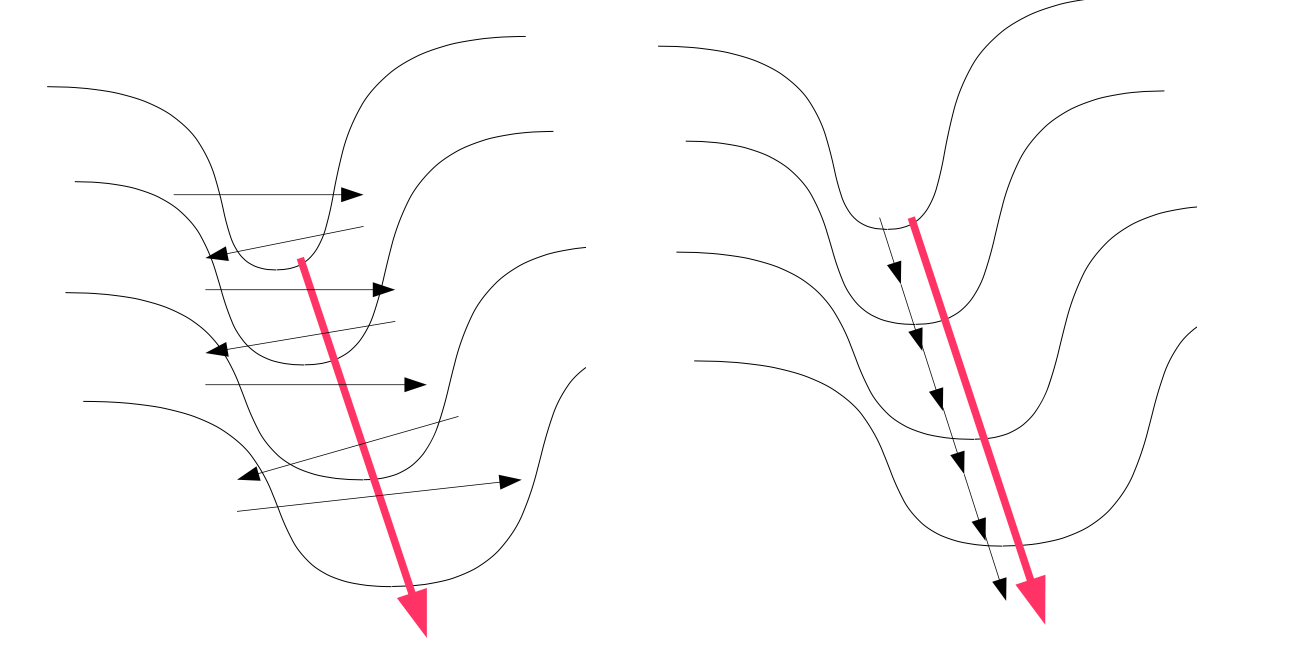
\includegraphics[scale=0.4]{curvature.png}
    \caption{Optimizing along a narrow valley}
    \label{}
  \end{figure}
  \end{frame}

  \subsection{Hessian-Free(HF) optimization}
	\begin{frame}
	  \frametitle{Hessian-Free(HF) optimization}
     The newton method implicitly solve the following linear system (\textbf{Newton's system}):
    \begin{equation}
      \nabla^{2} f(\underline{x}_k) \underline{d} = - \nabla f(\underline{x}_k)
      \label{newtonsys}
    \end{equation}
    \textbf{Idea}: Apply an iterative method for finding the solution of (\ref{newtonsys}).\newline\newline
    The iterative method is not run up to convergence but an approximate solution is accepted.

	\end{frame}

  \subsection{HF - Inner Algorithm}
  \begin{frame}
    \frametitle{Hessian Free and Conjugate Gradient - 1}
    A very common choice for the inner procedure is the \textbf{Conjugate Gradient Method}.\newline\newline
    CG is a very effecting algorithm for optimizing quadratic functions. \newline \newline

    In the worst case CG is guaranteed to converge in at most $n$ iterations it is impractical for very large problem
    to wait for CG to completely converge in general.\newline\newline

    In practice the behaviour of CG is that it will make significant improvements well before $n$ iterations.

    Moreover despite Quasi-Newton methods, HF does not make any approximation of the Hessian of the function!


  \end{frame}

  \subsection{Hessian Free and Conjugate Gradient - 2}
  \begin{frame}
    \frametitle{Hessian Free and Conjugate Gradient - 2}
    The classical CG method require some modifications:\newline\newline

    The standard CG algorithm is used to solve positive definite systems, but the Hessian
    of the function may have negative eigenvalues, so CG must stop as soon as a direction of negative curvature is generated.\newline\newline

    For every iteration of CG we require the following condition to be satisfied:
    \begin{enumerate}
      \item The starting point $d^{(0)} = \underline{0}$
      \item Curvature test. If CG generates a direction $d$ such that
        \begin{equation*}
          p^{t} \nabla^2 f(x_k) p < 0
        \end{equation*}

    \end{enumerate}

  \end{frame}

  \subsection{Hessian Free and Conjugate Gradient - 3}
	\begin{frame}
	  \frametitle{Hessian Free and Conjugate Gradient - 3}
    \indent Then if $k = 0$, we complete another iteration and then CG return the solution $d^{(k+1)}$,
    if $k > 0$ then we stop immediately and return $d^{(k+1)}$.
    \vspace{4cm}

	\end{frame}

  \subsection{Hessian Free - Convergence Rate}
  \begin{frame}
    \frametitle{Hessian Free - Convergence Rate}
    \textbf{Theorem 1}. Assume that $f$ is continuously differentiable in a neighborhood of a local solution $x^*$ of the original problem.
    In addition, assume that  $\nabla^{2} f(x^*)$ is nonsingular and that $\nabla f$ is Lipschitz continuous at $x^*$.\newline
    Assume that iteration k of the truncated-Newton method computes a step $p_k$ that satisfies:
    \begin{equation}
      || \nabla f{\underline{x}_k} + \nabla^2 f{\underline{x}_k} p_k || \leq \eta_{k} ||\nabla f(\underline{x}_k)||
    \end{equation}
    For a specified value of $\eta_k$; the new estimate of the solution is computed using $x_{k+1} \leftarrow x_k + p_k$. \newline
    If $x_0$ is sufficiently close to $x^*$ and $0 \leq \eta_k \leq \eta_{max} < 1$ then {$x_k$} converges to $x^*$ linearly in the norm $|| \cdot ||_{*}$ defined by
    $||v||∗ := ||\nabla^2 f(x^{*})v||$, with asymptotic rate constant no greater than $\eta_{max}$.\newline
  \end{frame}

  \subsection{Hessian Free - Convergence Rate}
  \begin{frame}
    \frametitle{Hessian Free - Forcing Sequences}
    If $\lim_{k \rightarrow \infty}  \eta_k = 0$; then the convergence is superlinear.\newline
    If  $k = O(||f(x_k)||^r)$ for $0 < r \leq 1$; then the convergence is of order at least $(1 + r)$.\newline\newline

    Common choice for $\eta_k$ (also known as \textit{Forcing Sequence}) are:
    \begin{equation*}
      \eta_{k} = \min{\{\frac{1}{2}, c ||\nabla f(x_k)||^{r}}\}
    \end{equation*}
    with $c \geq 0$ and $0 \leq r \leq 1$

  \end{frame}

  \subsection{Hessian Free + CG - Sketch Algorithm}
  \begin{frame}
    \frametitle{Hessian Free + CG - Sketch Algorithm}
    \begin{figure}
      \centering
      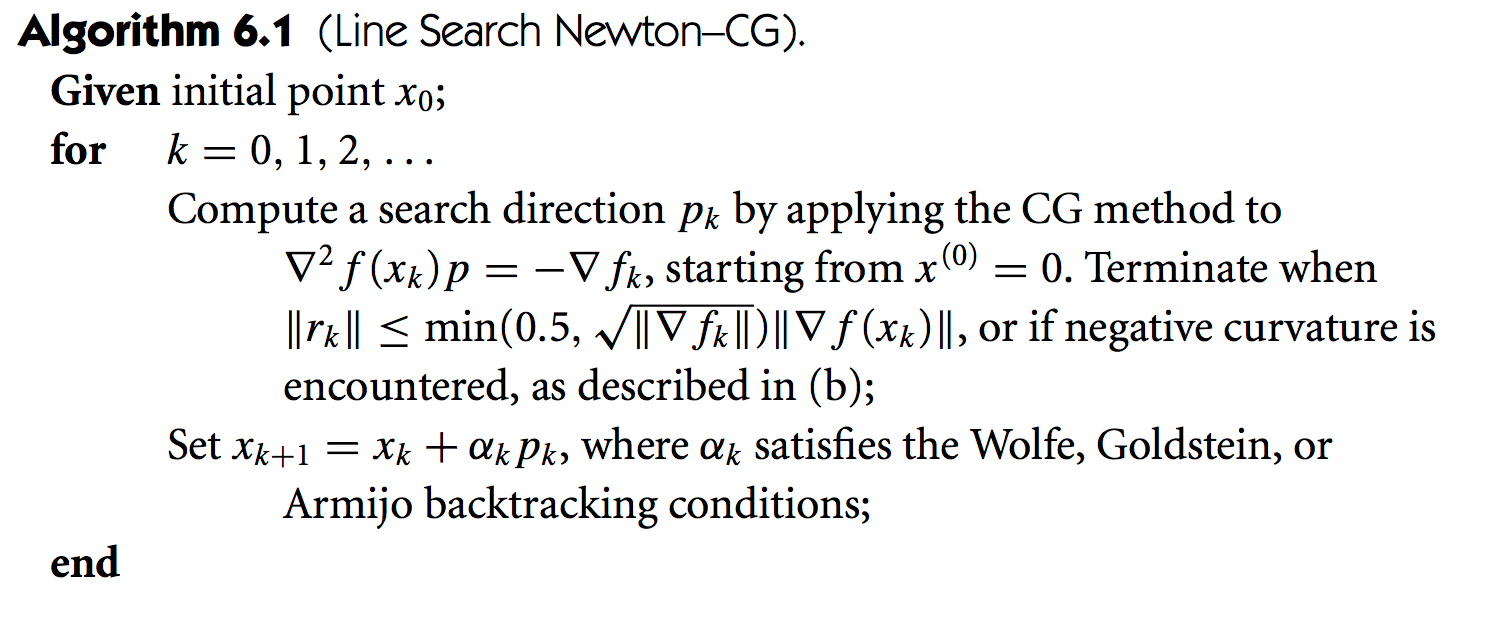
\includegraphics[scale=0.4]{algorithm.png}
      \caption{Sketch algorithm for HF+CG method}
      \label{}
    \end{figure}

  \end{frame}

  \subsection{Hessian Free + CG - Problems}
  \begin{frame}
    \frametitle{Hessian Free + CG - Problems}
    In practice the method results to be very slow when $\nabla^2 f(\underline{x}_k)$ is nearly
    singular. A trust-region approach is proposed to partially alleviate this problem.\newline\newline

    In the following the autor of \cite{martens} propose a series of optimization to effectively use HF+CG in
    machine learning settings:
    \begin{enumerate}
      \item Damping
      \item Matrix-vector Product
      \item Termination Conditions
      \item Preconditioning
    \end{enumerate}
  \end{frame}

  \subsection{Hessian Free + CG - Damping}
  \begin{frame}
    \frametitle{Hessian Free + CG - Damping}
    The idea is to use CG to solve:
    \begin{equation*}
      (\nabla^{2} f(\underline{x}_k) \underline{d} + \lambda \underline{d}) = - \nabla f(\underline{x}_k)
    \end{equation*}
    where $\lambda$ is the so-called damping factor. The exact curvature matrix available to HF allows
    for the identification of extremely low curvature directions.\newline\newline

    When such a direction is detected CG will elect to move far from along it and possibly well outside the region
    where the original quadratic approximation is a sensible approximation.\newline\newline

    $\lambda$ can be interpreted as controlling how \textit{conservative} the approximation is.
  \end{frame}

  \subsection{Hessian Free + CG - Matrix-Vector product}
	\begin{frame}
	  \frametitle{Hessian Free + CG - Matrix-Vector product}
      Let $\underline{d} \in \mathbb{R}^{n}$ and $H \in \mathbb{R}^{n \times n}$ then:
      \begin{equation*}
        H\underline{d} = \lim_{\epsilon \rightarrow 0} \frac{\nabla f(\underline{x}_k + \epsilon \underline{d}) - \nabla f{(\underline{x}_k)}}{\epsilon}
      \end{equation*}
      Using this formula the product can be calculated using only one extra evaluation of the gradient of $f$.\newline\newline
      Other techniques (with better numerical properties), in case complex arithmetic is available, permit an estimation that is accurate
      to $O(\epsilon)$.

	\end{frame}

  \subsection{Hessian Free + CG - Termination Condition}
	\begin{frame}
	  \frametitle{Hessian Free + CG - Termination Condition}
    The typical termination condition (as seen before) is of the type:
    \begin{equation}
      ||r_k|| \leq \min{\{ 0.5, ||\nabla f(x_k)||^{\frac{1}{2}}\}} ||\nabla f(x_k)||
    \end{equation}
    We use CG to solve $Ax = b$, but the method does not optimize $||Ax - b||^2$ but $\phi(x) = \frac{1}{2}x^{t} A x - b^{t}x$.
    In particular we choose $A = H(x)$ and $b = -\nabla f(x)$.\newline \newline

    One sub-optimal solution for one method may be terrible for the other.\newline
    In practice the authors of \cite{martens} found the following condition to be much more efficient:
    \begin{equation}
      i > k, \phi(x_i) < 0, \frac{\phi(x_i) - \phi(x_{i-k})}{\phi(x_i)} < k\epsilon
    \end{equation}
	\end{frame}

  \subsection{Hessian Free + CG - Preconditioning}
	\begin{frame}
	  \frametitle{Hessian Free + CG - Preconditioning}
    Preconditioning is a technique to accelerate CG.\newline
    We define a linear change of variables $\hat{x} = Px$.\newline
    The new quadratic objective is
    \begin{equation*}
      \hat{\phi}(\hat{x}) = \frac{1}{2} \hat{x}^{t} P^{-t} A P^{-1} \hat{x} - (P^{-1}b)^{t} \hat{x}
    \end{equation*}
    To use preconditioning one must specify $M := P^{t}P$ with the understanding that $My = x$ is easy to solve.\newline\newline

    A possible choice:
    \begin{equation}
      M = \left[ diag \left ( \sum_{i=1}^{D} \nabla f_{i}(x) \times \nabla f_{i}(x)\right ) + \lambda I \right ]^{\alpha}
    \end{equation}
  \end{frame}

  \subsection{Trust Region approach}
  \begin{frame}
    \frametitle{Trust Region approach}
    \textbf{Idea:} search for $\underline{d}_k$ and $\alpha_k$ at the current $x_k$ over a
    \textit{trust region} $B_k$.\newline
    Example: $B_k = \{\underline{x} \in \mathrm{R} : ||\underline{x} - x_k|| < \Delta_k\}$\newline

    This results in solving an additional problem referred as the \textit{trust-region subproblem}.\newline

    The subproblem in general can be solved in closed form or with low computational requirements.

    Moreover the size (or radius) of the trust region is changed adaptively at each iteration.
  \end{frame}

  \subsection{Trust Region - Subproblem}
  \begin{frame}
    \frametitle{Trust Region - Subproblem}
    The trust region subproblem is generally defined as:
    \begin{equation}
      \min_{\underline{d} \in \mathbb{R}^n} \{m_k(\underline{d}) := f_k + \nabla f_k^{t} x + \frac{1}{2} d^{t} B_k d \} \quad st \quad ||d|| < \Delta_k
      \label{subproblem}
    \end{equation}

    Specifically for the Newton-CG method the computation step consists in setting $B_k = \nabla^2 f(x_k)$ and
    applying the CG procedure to:

    \begin{equation*}
      B_k d_k = - \nabla f_k
    \end{equation*}
    and stopping if:
    \begin{itemize}
      \item The size (norm) of the solution exceeds the $\Delta_k$.
      \item The system has been solved to a required accuracy.
      \item Negative curvature condition is reached.
    \end{itemize}
  \end{frame}

  \subsection{Trust Region - Properties}
  \begin{frame}
    \frametitle{Trust Region - Properties}
    The Trust-Region Newton-CG method has a number of desirable properties:
    \begin{itemize}
      \item It is \textbf{globally convergent}: the first step along the direction $-\nabla f_k$ identifies
        the Cauchy point of \ref{subproblem} and the subsequent directions only improves the model value.
      \item It requires no matrix factorizations, so we can exploit the sparsity structure of the Hessian
        without worrying about fill-in during a direct factorization.
      \item The CG iteration, the most computationally intensive part of the algorithm, may be executed in parallel
        since the key operation is a matrix-vector product.
    \end{itemize}
  \end{frame}

  \subsection{Trust Region - Properties}
  \begin{frame}
    \frametitle{Trust Region - Properties}
    \begin{itemize}
      \item When the Hessian matrix is positive definite, the Newton-CG method approximates the pure Newton step
        more and more closely as the solution $x^*$ is approached, so rapid convergence is also possible.
      \item Two advantages, compared with the line search Newton-CG method, are that the lengths of the steps are
        controlled by the trust region and that directions of negative curvature are often explored.
      \item A limitation of the trust-region Newton-CG method is that it accepts any direction of negative curvature,
        even when this direction gives an insignificant reduction in the model.
    \end{itemize}
    The limitation is overcome by the \textbf{Lanczos method}; the idea is to solve (\ref{newtonsys}) but it
    does not stop at the first negative curvature direction but continues in search for a sufficiently negative
    curvature direction.
  \end{frame}

  \subsection{Deep Learning - Introduction}
  \begin{frame}
    \frametitle{Deep Learning - Introduction}
    Deep learning can be summarized as learning both the representation and the classifier out of it.
    \begin{figure}
      \centering
      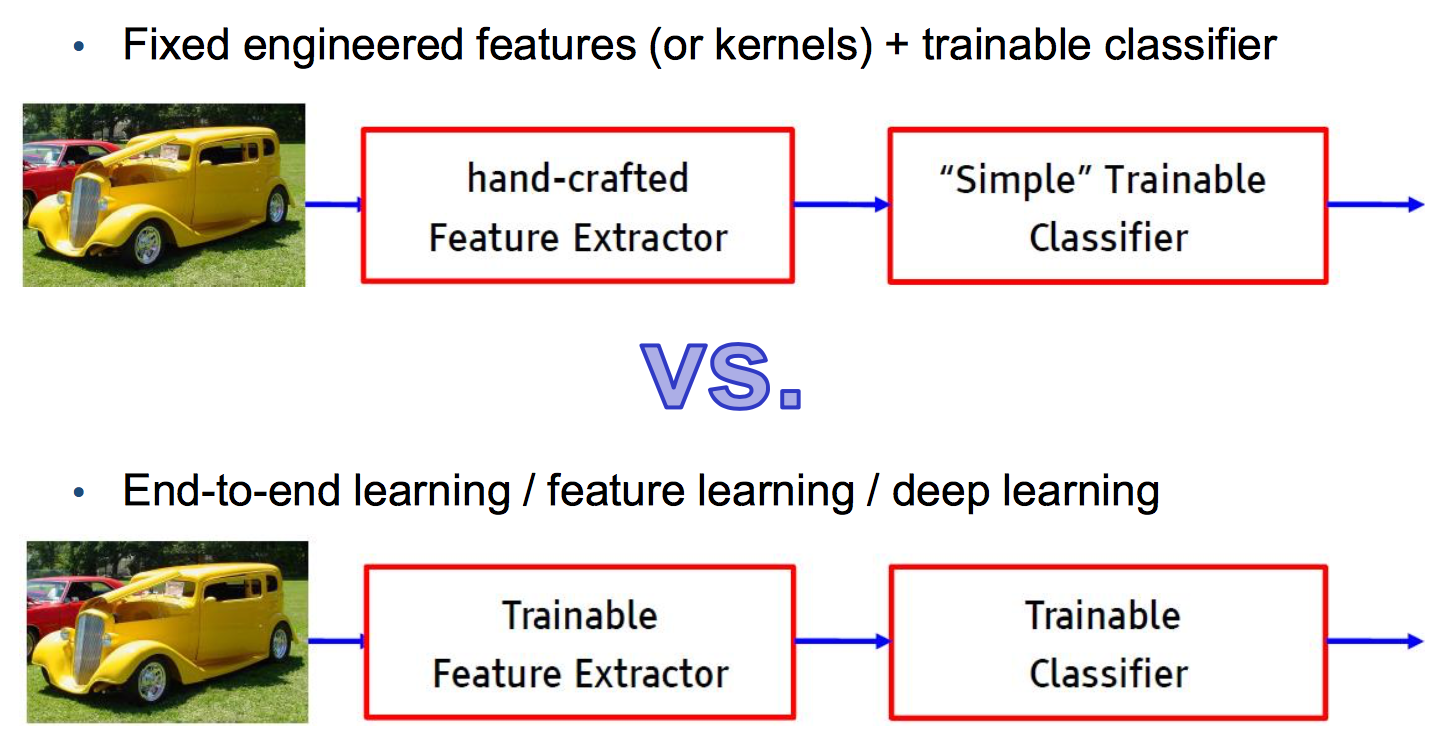
\includegraphics[scale=0.4]{deep1.png}
      \label{}
    \end{figure}
  \end{frame}

  \subsection{Deep Learning - Representation}
  \begin{frame}
    \frametitle{Deep Learning - Representation}
    In deep learning we have multiple stages of non linear feature trasformation
    \begin{figure}
      \centering
      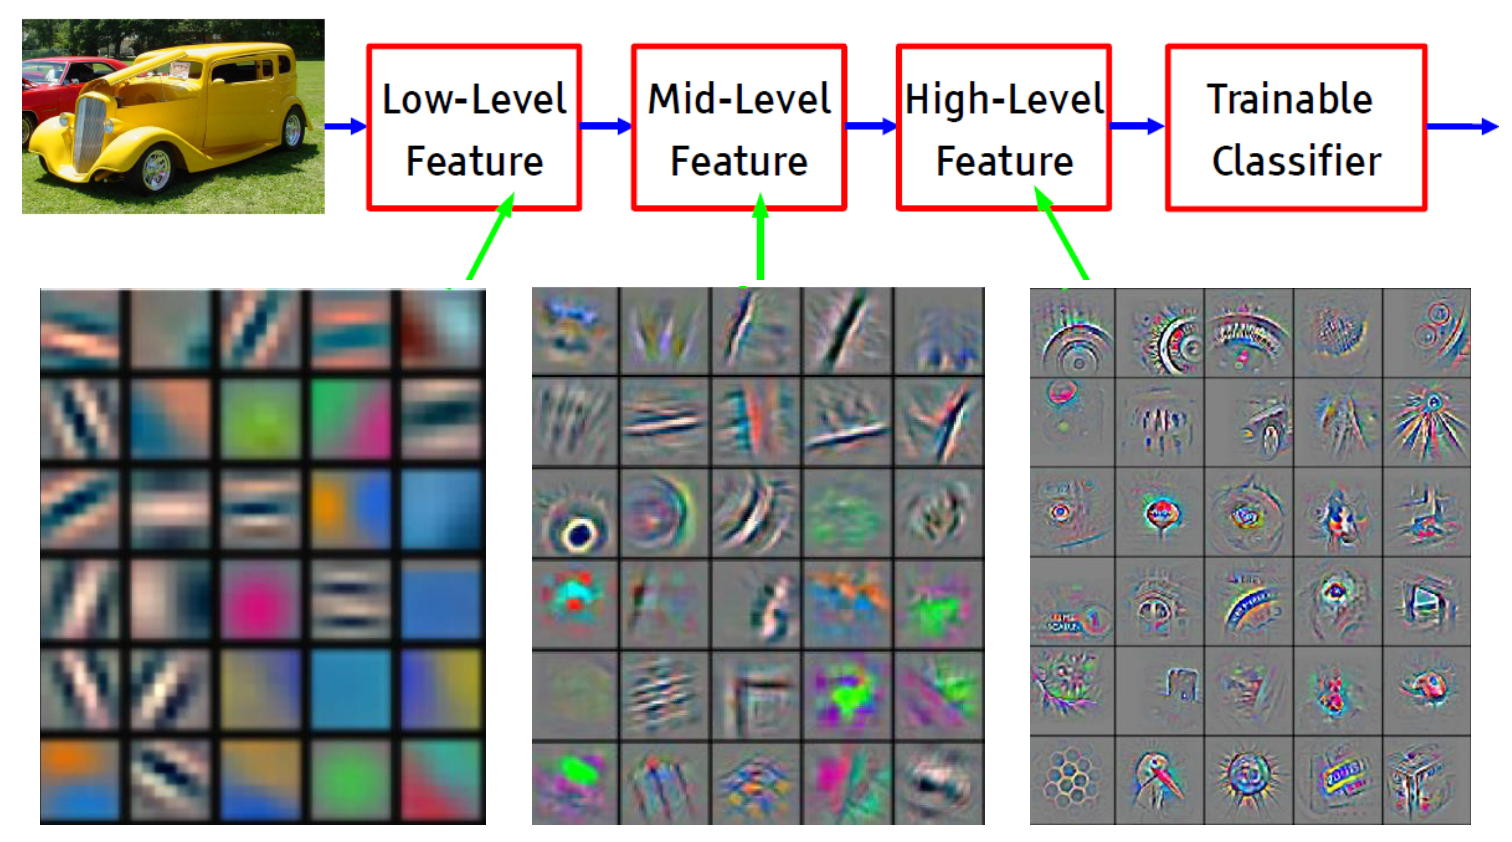
\includegraphics[scale=0.4]{deep2.png}
      \label{}
    \end{figure}
  \end{frame}

  \subsection{Deep Learning - Trainable features hierarchy}
  \begin{frame}
    \frametitle{Deep Learning - Trainable features hierarchy}
    Deep learning assumes it is possible to \textit{learn} a hierarchy
    of descriptors with increasing abstraction.
    \begin{figure}
      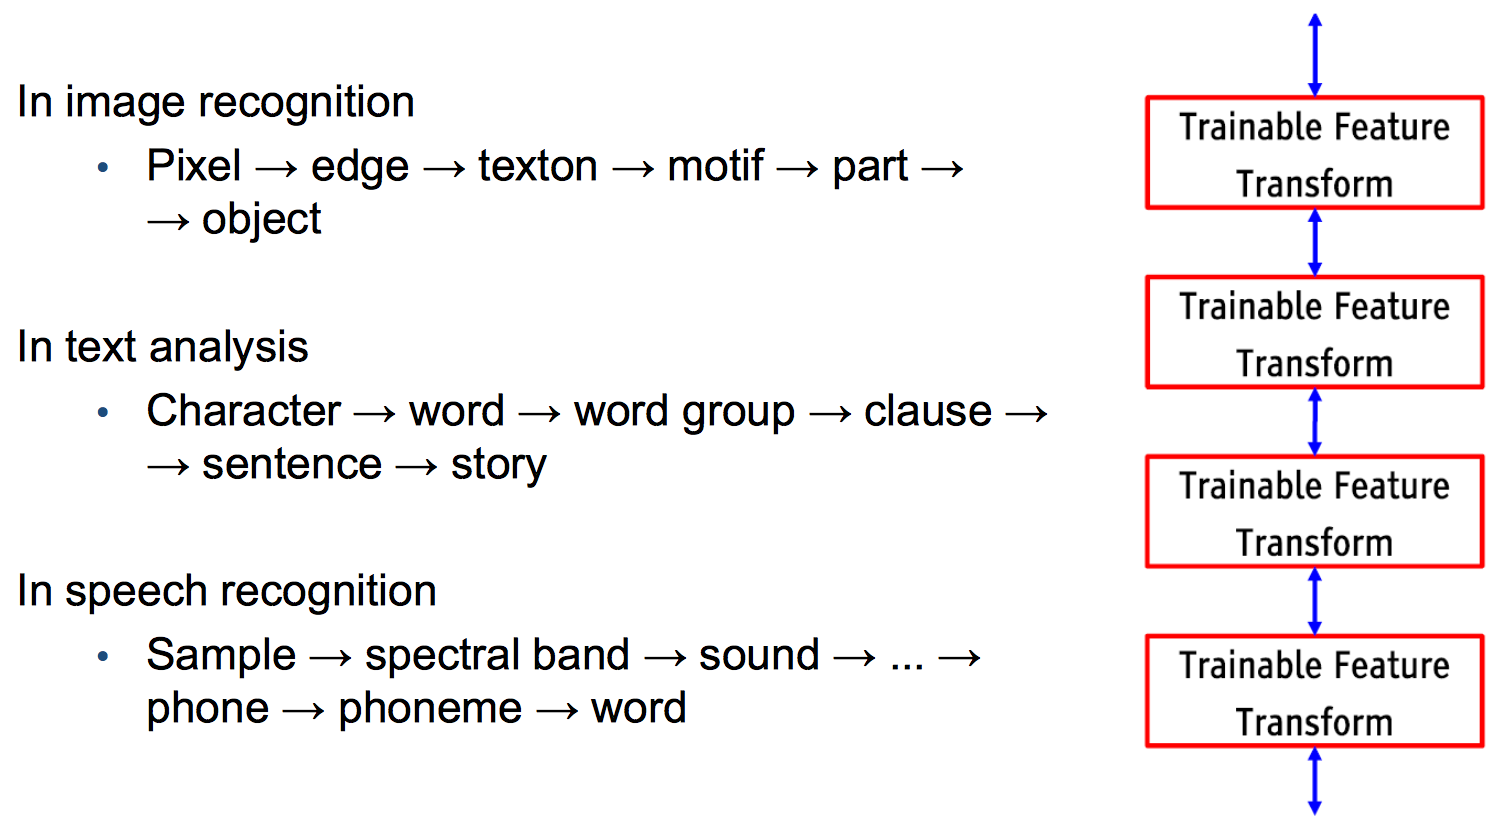
\includegraphics[scale=0.4]{deep3.png}
      \label{}
    \end{figure}
  \end{frame}

  \subsection{Deep Learning - Architectures}
  \begin{frame}
    \frametitle{Deep Learning - Architectures}
    \mbox{}\hfill\raisebox{-\height}[0pt][0pt]{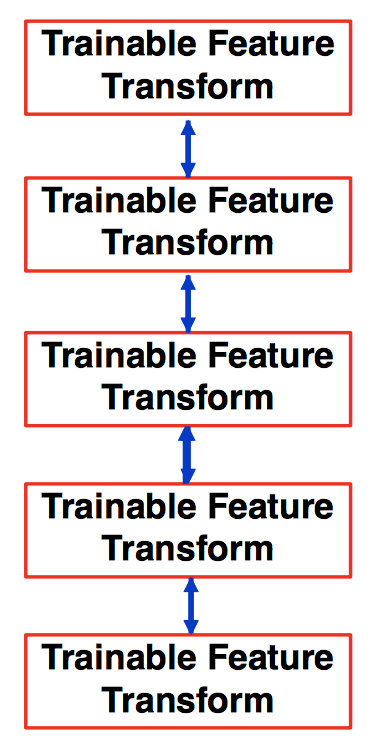
\includegraphics[width=.25\linewidth]{deep4.png}}
    \vspace*{-\baselineskip}


    Depending on the direction of the information flow we can have different architectures for the hierarchy of features
    \begin{itemize}
      \item \lenitem{Feed forward (e.g., multilayer neural nets, convolutional nets, etc.)}
      \item \lenitem{Feed back (e.g., Stacked sparse coding, Deconvolutional nets, etc.)}
      \item \lenitem{Bi-directional (e.g, Deep Boltmann Machines, \textbf{Stacked Auto-Encoders}, etc.)}
    \end{itemize}
    Associated with different types of learning
    protoc- \newline ols (supervised, semi-supervised, self-taught, etc.)
  \end{frame}



  \subsection{Experiments - Autoencoders}
	\begin{frame}
    \frametitle{Experiments - Autoencoders}
    Given an unlabelled dataset $\{x^{(i)}\}_{i=1}^m$, an auto encoder is a two-layer neural
    network that learns non-linear codes to represents (or reconstruct) the data.\newline\newline

    Specifically we want to learn $h(x^{(i)}; W, b) = \sigma(Wx^{(i)} + b)$ such that $\sigma(W^{t} h(x^{(i)}; W, b) + c)$
    is approximately $x^{(i)}$. That is:
    \begin{equation*}
      \min_{W,b,c} \sum_{i=1}^{m} ||\sigma(W^{t} h(x^{(i)}; W, b) + c) - x^{(i)}||_{2}^{2}
    \end{equation*}
  \end{frame}

  \subsection{Experiments - Autoencoders - 2}
  \begin{frame}

    \frametitle{Experiments - Autoencoders - 2}
    \begin{figure}
      \centering
      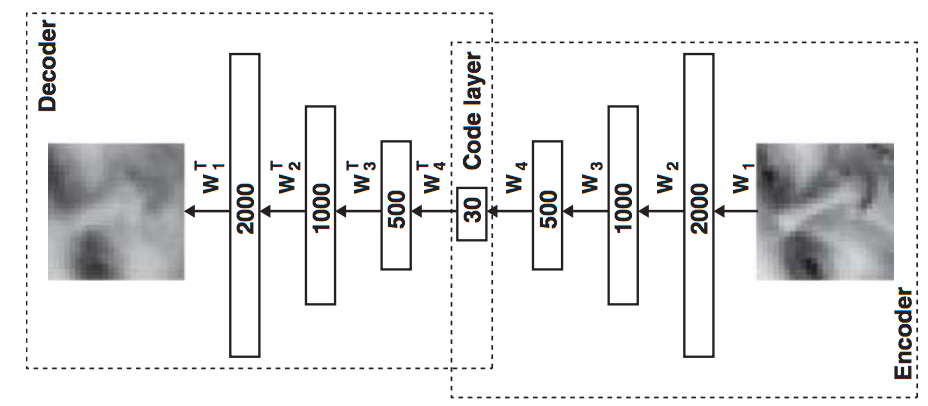
\includegraphics[scale=0.6]{autoenc.png}
      \caption{A stacked autoenconder}
      \label{}
    \end{figure}
  \end{frame}

  \subsection{Experiments - Autoencoders - Results}
  \begin{frame}
    \frametitle{Experiments - Autoencoders - Parameters}
    \begin{figure}
      \centering
      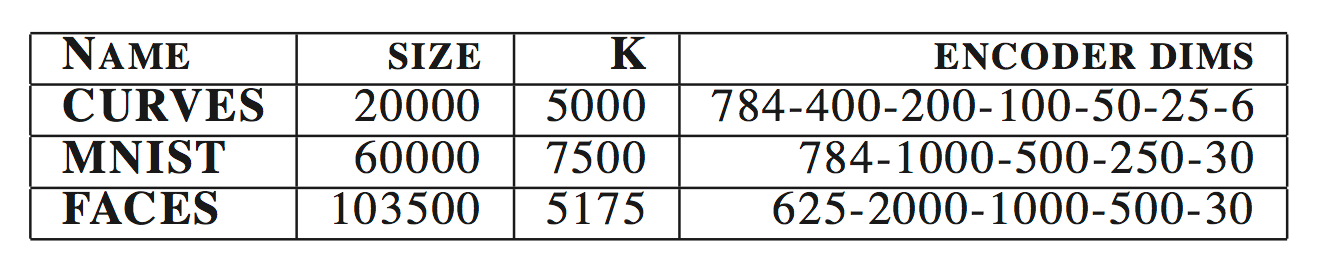
\includegraphics[scale=0.4]{parameters.png}
      \caption{Parameters for different datasets}
      \label{}
    \end{figure}
    \begin{figure}
      \centering
      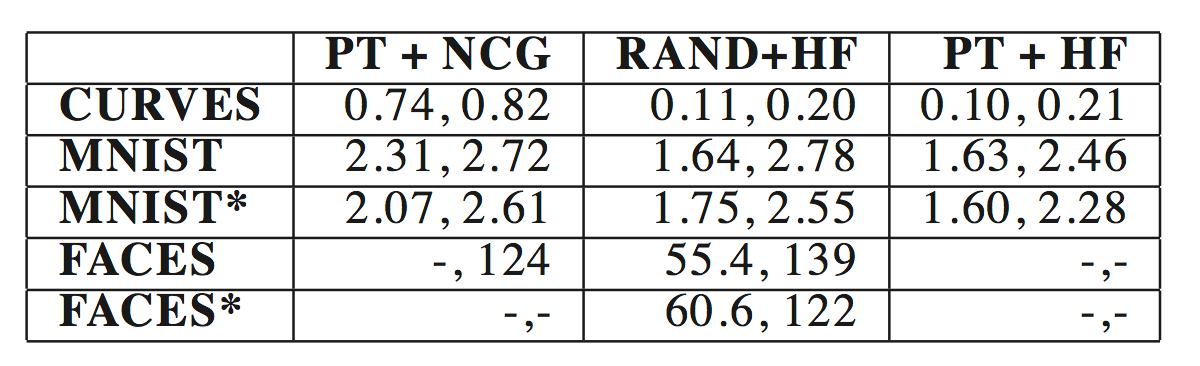
\includegraphics[scale=0.4]{res1.png}
      \caption{Results for different datasets}
      \label{}
    \end{figure}

  \end{frame}

  \subsection{Experiments - Autoencoders - Timings}
  \begin{frame}
    \frametitle{Experiments - Autoencoders - Timings}
    \begin{figure}
      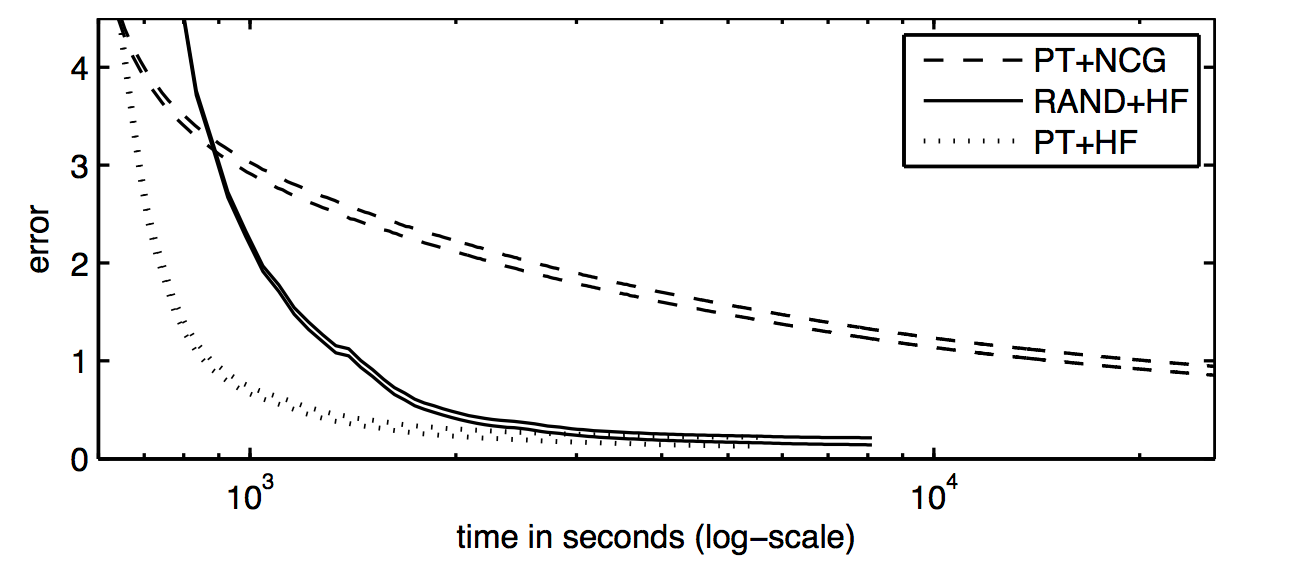
\includegraphics[scale=0.4]{res2.png}
      \caption{Timing for diffrent methods and datasets}
      \label{}
    \end{figure}

  \end{frame}

  \subsection{Experiments - Autoencoders - Discussion}
  \begin{frame}
    \frametitle{Experiments - Autoencoders - Discussion}
    The most important implications is that the authors have been able to learn a deep-model
    with a completely generic optimizer without \textbf{the need of pretraining}.\newline

    A clear theme that emerges from the results is that HF optimized nets have a much lower training error,
    implying that the HF approach is more effective than pre-training $+$ fine-tuning.\newline

    The pre-trained version of HF benefits in terms of speed of convergence but does not gain any significant
    advantage in terms of underfitting.\newline

    It is clear that pre-training helps $1^{st}$ approximation algorithm in overcoming the underfitting problem by
    placing the parameter in a region less affected by the pathological-curvature scenario.
  \end{frame}

  \subsection{bibliography}
  \begin{frame}
    \frametitle{References}
    \begin{thebibliography}{9}
      \bibitem{martens}
      Martens, James. \emph{Deep learning via Hessian-free optimization.}
      Proceedings of the 27th International Conference on Machine Learning (ICML-10). 2010.

    \bibitem{ng}
      Ngiam, Jiquan, et al. \emph{On optimization methods for deep learning.}
      Proceedings of the 28th international conference on machine learning (ICML-11). 2011.

    \bibitem{nocedal}
      Wright, Stephen J., and Jorge Nocedal.
      \emph{Numerical optimization.}
      Springer Science 35.67-68 (1999): pages 139-142.

    \bibitem{hilton}
    Hinton, Geoffrey E., and Ruslan R. Salakhutdinov.
    \emph{Reducing the dimensionality of data with neural networks.}
     Science 313.5786 (2006): pages 504-507.
    \end{thebibliography}
  \end{frame}

\end{document}
